\documentclass[11pt,a4paper]{article}

\usepackage{amsmath}
\usepackage{hyperref}
\usepackage{lipsum}
\usepackage{listings}
\usepackage{tikz}

\title{\LaTeXe{} Example Document}
\author{Frank Jung}
\date{29 Jul 2016}

\begin{document}

\pagenumbering{gobble}
\maketitle
\newpage

\pagenumbering{roman}
\tableofcontents{}
\listoffigures
% \listoftables
\newpage

\pagenumbering{arabic}
\newpage

\newcommand{\sectionbreak}{\clearpage}

\section*{Introduction}
\addcontentsline{toc}{section}{Introduction}

This is a \LaTeXe{} document to provide some examples of usage. To fill out the
document there are \href{http://www.lipsum.com/}{Lorem Ipsum} paragraphs.

\lipsum[1]

\sectionbreak{}

\section*{Equations}
\addcontentsline{toc}{section}{Equations}

Equations can be included into the document in a number of ways. The first
example can be a either number or unnumbered equation.

\paragraph{}
The mass-energy equivalence is described by the famous equation:

\begin{equation}
  E = mc^2
\end{equation}

\paragraph{}
Equations can also be inline. For example, $f(x) = x^2$. An more text here.
\lipsum[2]

\sectionbreak{}

\section*{Gnuplot}
\addcontentsline{toc}{section}{Gnuplot}

Plots can be included or rendered inline. The following example uses
\href{http://www.gnuplot.info/}{Gnuplot} to graph functions.

\subsection*{Inline Gnuplot}
\addcontentsline{toc}{subsection}{Inline Gnuplot}

To render this inline plot ensure that:
\begin{itemize}
  \item \texttt{gnuplot} is installed
  \item \texttt{latexmf} requires the \texttt{-shell-escape} option
\end{itemize}
This renders as:

\begin{figure}[h]
  \centering
  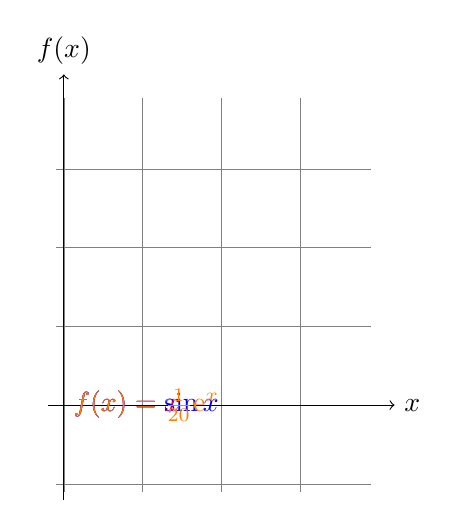
\begin{tikzpicture}[domain=0:4]
    \draw[very thin,color=gray] (-0.1,-1.1) grid (3.9,3.9);
    \draw[->] (-0.2,0) -- (4.2,0) node[right] {$x$};
    \draw[->] (0,-1.2) -- (0,4.2) node[above] {$f(x)$};
    \draw[color=red] plot[id=x] function{x}
      node[right] {$f(x) =x$};
    \draw[color=blue] plot[id=sin] function{sin(x)}
      node[right] {$f(x) = \sin x$};
    \draw[color=orange] plot[id=exp] function{0.05*exp(x)}
      node[right] {$f(x) = \frac{1}{20} \mathrm e^x$};
  \end{tikzpicture}
  \caption{Inline Gnuplot example}
\end{figure}
The code to generate this plot is:
\lstset{basicstyle=\footnotesize\ttfamily}
\begin{figure}[h]
  \begin{lstlisting}[frame=single,language=TeX,tabsize=2,numbers=left,numberstyle=\tiny]
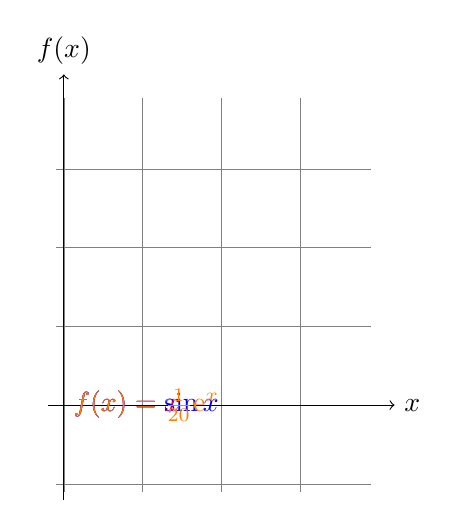
\begin{tikzpicture}[domain=0:4]
  \draw[very thin,color=gray] (-0.1,-1.1) grid (3.9,3.9);
  \draw[->] (-0.2,0) -- (4.2,0) node[right] {$x$};
  \draw[->] (0,-1.2) -- (0,4.2) node[above] {$f(x)$};
  \draw[color=red] plot[id=x] function{x}
    node[right] {$f(x) =x$};
  \draw[color=blue] plot[id=sin] function{sin(x)}
    node[right] {$f(x) = \sin x$};
  \draw[color=orange] plot[id=exp] function{0.05*exp(x)}
    node[right] {$f(x) = \frac{1}{20} \mathrm e^x$};
\end{tikzpicture}
  \end{lstlisting}
  \caption{LaTeX snippet for embedded Gnuplot}
\end{figure}

\pagebreak[1]

\subsection*{External Gnuplot}
\addcontentsline{toc}{subsection}{External Gnuplot}

This example includes an externally rendered Gnuplot.

\begin{figure}[h]
  \centering
  \includegraphics{plot}
  \caption{External Gnuplot example}
\end{figure}

The code to generate this plot is:
\lstset{basicstyle=\footnotesize\ttfamily}
\begin{figure}[h]
  \begin{lstinputlisting}[frame=single,language=Gnuplot,tabsize=2,numbers=left,numberstyle=\tiny]{plot.gnuplot}
  \end{lstinputlisting}
  \caption{Gnuplot source code}
\end{figure}

\pagebreak[4]

\section*{Makefile}
\addcontentsline{toc}{section}{Makefile}

This project use a \href{https://www.gnu.org/software/make/}{Makefile} to build
a PDF from this document. The Makefile is very simple:

\begin{figure}[h]
  \lstset{basicstyle=\footnotesize\ttfamily}
  \lstinputlisting[frame=single,language=make,tabsize=4,showspaces=false,numbers=left,numberstyle=\tiny]{Makefile}
  \caption{Makefile source code}
\end{figure}

\end{document}
